% 连续叉乘的化简
% 线性代数|矢量|叉乘|cross product|叉积|cross product|向量积|vector product|矢量积

\pentry{矢量的叉乘\upref{Cross}}

连续两个叉乘的化简也叫 BAC-CAB 定理
\begin{gather}
\bvec A \cross (\bvec B \cross \bvec C) = \bvec B (\bvec A \vdot \bvec C) - \bvec C (\bvec A \vdot \bvec B)\label{TriCro_eq1}\\
(\bvec B \cross \bvec C) \cross \bvec A = \bvec C (\bvec A \vdot \bvec B) - \bvec B (\bvec A \vdot \bvec C)
\end{gather}

要证明这个定理可以将每个叉乘在各个基底上展开(\autoref{Cross_eq2}~\upref{Cross}).

\begin{exercise}{}
由叉乘的坐标定义(\autoref{Cross_eq2}~\upref{Cross}) 证明\autoref{TriCro_eq1}.
\end{exercise} 

这里对连续叉乘的几何意义略作说明, 可以用于理解该公式的结构. 以\autoref{TriCro_eq1} 为例, 根据叉乘的几何意义我们知道 $\bvec B \cross \bvec C$ (命名为 $\bvec D$) 方向垂直于 $\bvec B$ 和 $\bvec C$ 所在平面. 又因为 $\bvec A \cross \bvec D$ 垂直于 $\bvec D$, 所以最终的矢量再次落到 $\bvec B$ 和 $\bvec C$ 所在平面上, 所以等式右边是 $\bvec B$ 和 $\bvec C$ 的线性组合.

下面来介绍一种简单的记忆方法,括号外的矢量在哪边, 括号内靠近那边的矢量所在的项前面就是正号,另一项前面则是负号,如\autoref{TriCro_fig1} 所示.

\begin{figure}[ht]
\centering
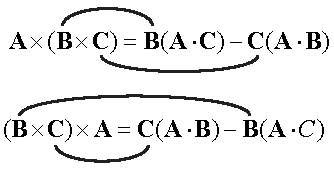
\includegraphics[width=6cm]{./figures/TriCro_1.pdf}
\caption{三矢量叉乘的化简}\label{TriCro_fig1}
\end{figure}